\documentclass[aspectratio=169,xcolor=table]{beamer}
%aspcetratio >> 1610 169 149 54 43 32
%The themes:
\usetheme[style=classic]{mharvellous}
%\usetheme[style=dark]{mharvellous}
%\usetheme[style=mracula]{mharvellous}
% \usetheme[style=default]{mharvellous}
%*--------------------------------------------------
%\usepackage{helvet}
%*--------------------------------------------------
\usepackage{bibunits}  
%\setbeamertemplate{bibliography item}{[\theenumiv]}
\setbeamertemplate{bibliography item}{\insertbiblabel}
\defaultbibliography{bibliography}
%\defaultbibliographystyle{IEEEtran}
%\defaultbibliographystyle{amsalpha}
\defaultbibliographystyle{abntex2-alf}
%\bibliography{bibliography}
%\usepackage[backend=biber,style=alphabetic,citestyle=authoryear]{biblatex}
% \addbibresource{bibliography.bib}
%\usepackage{natbib}
\usepackage{bibentry}
%*--------------------------------------------------
\usepackage{lipsum}
\usepackage{epigraph}
\usepackage{graphicx}
\usepackage{multirow}
%\usepackage{enumitem}
\usepackage{array}
%\usepackage{multimedia}
\usepackage{media9}
%\usepackage{pdfpc-movie}
\usepackage{circledsteps}
\usepackage{listings}
\usepackage[normalem]{ulem}
%\usepackage{Sweave}
%\usepackage{xkeyval}
%\usepackage{palatino}
%\usepackage{pgfpages}
\usepackage{float}
%*--------------------------------------------------
\usepackage[timeinterval=1]{tdclock}
%\usepackage[font=Times,timeinterval=1, timeduration=200,resetatpages=all]{tdclock}
%\usepackage[font=Times,timeinterval=10, timeduration=2.0, timedeath=0, fillcolorwarningsecond=white!60!yellow,timewarningfirst=50,timewarningsecond=80,resetatpages=2]{tdclock}
%*--------------------------------------------------
\usepackage{url}
\usepackage{tabularx,booktabs}
\usepackage{threeparttable}
\usepackage[absolute, overlay]{textpos}
%*--------------------------------------------------
\usepackage{framed, color}
\usepackage[tikz]{bclogo}
\usepackage{spot}
\setspotlightcolor{red!50}
\usepackage{svg}
% %\setspotlightstyle{star, fill=red!50}
% %\setspotlightstyle{star points=7}
\usepackage{color,soul}
%\usepackage{xcolor}
\usepackage{tcolorbox}
\usepackage{xcolor}
\usepackage[export]{adjustbox}
\usepackage{verbatim}
\usetikzlibrary{trees,shapes,arrows}
\usepackage{fancyvrb}
\usepackage{float}
%*--------------------------------------------------
\usepackage{amsmath}
\usepackage{xfrac}
\usepackage{units}
\usepackage{ulem}
%*-------------------------------------------------------------------------------
%\newcolumntype{C}[1]{>{\centering\arraybackslash}m{#1}}
\newcolumntype{L}[1]{>{\raggedright\let\newline\\\arraybackslash\hspace{0pt}}m{#1}}
\newcolumntype{C}[1]{>{\centering\let\newline\\\arraybackslash\hspace{0pt}}m{#1}}
\newcolumntype{R}[1]{>{\raggedleft\let\newline\\\arraybackslash\hspace{0pt}}m{#1}}
%*-------------------------------------------------------------------------------
%\pgfpagesuselayout{2 on 1}[a4paper,border shrink=5mm]
%\setbeamertemplate{note page}[plain]
%\setbeameroption{show notes on second screen=bottom}
%*-------------------------------------------------------------------------------
\setbeameroption{hide notes}
%\setbeameroption{show only notes}
%\setbeameroption{show notes on second screen=right}
\setbeamertemplate{note page}{\pagecolor{yellow!5}\insertnote}
%*-------------------------------------------------------------------------------

%*-------------------------------------------------------------------------------
\title              {Snappy data storage}
\subtitle           {Dispositivo de armazenamento de dados mecânico}
\author             {João Vitor S. Mendes}
\email              {vitormendesrb@gmail.com}
\advisor            {Orientador: Marco A. dos Reis}
\institute          {Robótica e Sistemas Autônomos, Senai Cimatec}
\date               {Junho de 2022}
% \ulogo        		{Template/logosenaicimatecnegativo}
% \ulogof             {Template/logosenaicimatec2020}
% \ulogoo        		{Template/rosa-logo}
% \ulistelement    	{Template/bullet-white}

%*-------------------------------------------------------------------------------
\graphicspath{{source/pictures/}}
%*-------------------------------------------------------------------------------
\totalNoSlidesDisabled % To turn off the total number of slides in the footer. Comment this if you want the total number of slides in the footer
%*-------------------------------------------------------------------------------
\begin{document}
%*----------- COVER -------------------------------------------------------------
 \begin{frame}[t,plain]
%*----------- sound--------------------------------
    \includemedia[
        %width=1ex,
        %height=1ex,
        %activate=pageopen, 
        activate=onclick,
        deactivate=onclick,
        %passcontext,
        transparent,
        addresource=./source/sounds/hip-hop.mp3,
        flashvars={
                    source=./source/sounds/hip-hop.mp3
                    %&autoPlay=true
                    &autoRewind=true
                    &Play=2s
                    &repeat=always
                    %&Loop=true
        }
    ]
    {}{VPlayer.swf}
%*----------- start-page--------------------------
    \titlepage
    %*----------- notes-------------------------------
    \note[item]{Notes can help you to remember important information. Turn on the notes option.}
\end{frame}
%-
%*----------- SECTIONS ----------------------------------------------------------
%*----------- SLIDE -------------------------------------------------------------
\begin{frame}
    %\transdissolve[duration=0.5]
    %\hspace*{-1cm}
    \begin{columns}
        %\column{.01\textwidth}
        \column{0.4\textwidth}
        ~\hfill
        \vbox{}\vskip-1.4ex%
        \begin{beamercolorbox}[sep=8em, colsep*=18pt, center, wd=\textwidth, ht=\paperheight]{title page header}%
            \begin{center}
                \textbf{\huge{Introdução}}
            \end{center}
        \end{beamercolorbox}%
        \hfill\hfill
        \column{.05\textwidth}
        \column{.6\textwidth}
    \begin{figure}[H]
        \centering
        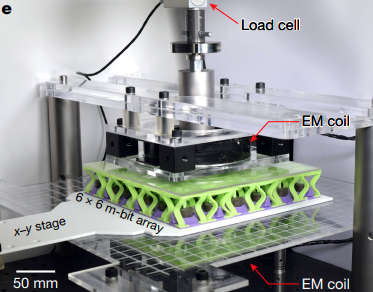
\includegraphics[scale = 0.5]{source/pictures/device.png}
        \caption{Imagem do dispositivo\cite{chen2021reprogrammable}.}
        \label{fig:device}
    \end{figure}

    \end{columns}

    %*----------- notes__
    \note[item]{Notes can help you to remember important information. Turn on the notes option.}
\end{frame}


\begin{frame}[t]{Introdução}
    \transboxout[duration=0.5]
    \begin{columns}
        \column{.2\textwidth}
    \end{columns}

    \begin{block}{O que é este dispositivo?}
    \only<2->{
        É um sistema de memória desenvolvido por \textit{Chen et al.} capaz manipular informações de forma mecânica\cite{coulais2021snappy}.}
    \end{block}
    \only<3->{
    O dispositivo é capaz de:
    \begin{itemize}
        \item Codificar
        \item Armazenar
        \item Ler
    \end{itemize}
    \only<4->{
    A informação codificada é capaz de determinar as propriedades mecânicas do dispositivo.}
    }
\end{frame}

\begin{frame}[t]{Introdução}
    \transboxout[duration=0.5]
    \textcolor{red}{Conceitos importantes}

    \begin{block}{O que é este dispositivo?}

        É um \Circled[outer color=red, inner ysep=8pt]{sistema de memória} desenvolvido por \textit{Chen et al.} capaz manipular informações de forma \Circled[outer color=red, inner ysep=8pt]{mecânica}\cite{coulais2021snappy}.
    \end{block}

    O dispositivo é capaz de:
    \begin{itemize}
        \item Codificar
        \item Armazenar
        \item Ler
    \end{itemize}

    A informação codificada é capaz de determinar as propriedades mecânicas do dispositivo.
    
\end{frame}


\begin{frame}[t]{Introdução}
    \transboxout[duration=0.5]
    \framesubtitle{Metamateriais}
    \begin{columns}
        \column{.1\textwidth}
        \column{.4\textwidth}
            \includegraphics[width=.87\textwidth]{hdd.png}
        \column{.6\textwidth}
            \begin{itemize}
                \item Apresenta funcionamento semelhante ao SDS\footnote{Snappy Data Storage}
                \item Utiliza \textit{bits} magneticos para manipular a informação
            
            \end{itemize}
    \end{columns}
   
\end{frame}



%-
%*----------- SLIDE -------------------------------------------------------------
\begin{frame}[c]{Introdução} 
    \transdissolve[duration=0.5]
   
    \begin{center}
        \Wider{%
        \begin{shaded}
        \begin{center}
            \vspace*{0.5cm}
            \resizebox{!}{0.7cm}{%
                \color{bg} Como funciona este dispositivo?
            }%
        \end{center}
        \end{shaded}
        }%
    \end{center}
    
   
%*----------- notes
    \note[item]{Notes can help you to remember important information. Turn on the notes option.}
\end{frame}
%-

%*----------- SLIDE -------------------------------------------------------------
\begin{frame}[t]{Sistemas de memória}
    \transboxout[duration=0.5]
    \framesubtitle{Hard Drives}
    \begin{columns}
        \column{.1\textwidth}
        \column{.4\textwidth}
            \includegraphics[width=.87\textwidth]{hdd.png}
        \column{.6\textwidth}
            \begin{itemize}
                \item Apresenta funcionamento semelhante ao SDS\footnote{Snappy Data Storage}
                \item Utiliza \textit{bits} magneticos para manipular a informação
            
            \end{itemize}
    \end{columns}
   
\end{frame}

\begin{frame}[t]{Sistemas de memória}
    \transboxout[duration=0.5]
    \framesubtitle{Funcionamento de um HD}    %\transboxin[duration=1,direction=30]

    \begin{figure}[H]
        \centering
        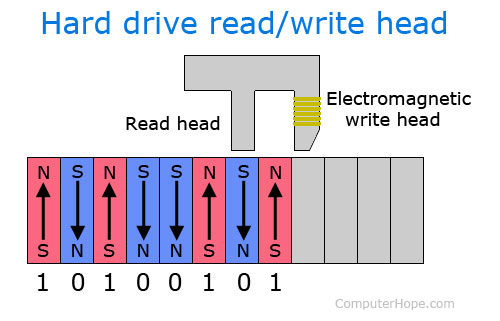
\includegraphics[scale = 0.40]{source/pictures/magnetic-media.jpg}
        \caption{Processo de gravação de dados em um disco rígido\cite{hdd-image}.}
        \label{fig:device}
    \end{figure}
%*----------- notes
    \note[item]{Notes can help you to remember important information. Turn on the notes option.}
\end{frame}

\begin{frame}[t]{Introdução}
    \transboxout[duration=0.5]
    \begin{columns}
        \column{.2\textwidth}
    \end{columns}

    \begin{block}{Bits}
        Unidades básicas de armazenamento do sistema de memória. É possível comparar a funcionalidade dos bits magnéticos com os bits mecânicos.
    \end{block}
    \only<2->{
    \begin{alertblock}{Mas, o que são esses bits mecânicos?}
    \end{alertblock}
    }
\end{frame}

\begin{frame}[t]{Unidade básica de armazenamento}
    \transboxout[duration=0.5]
    \framesubtitle{Shell - Bits mecânicos}
    \begin{columns}
        \column{.1\textwidth}
        \column{.4\textwidth}
            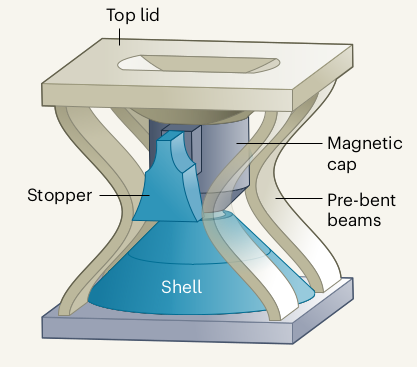
\includegraphics[width=.87\textwidth]{shell.png}
        \column{.6\textwidth}
            \begin{itemize}
                \item Conchas\footnote{Tradução livre de \textit{shell}.} que possuem uma instabilidade no seu encaixe.
                \item O encaixe pode ser controlado remotamente por um campo magnético externo.
            
            \end{itemize}
    \end{columns}
    
    \note[item]{Somente duas posições possuem estabilidade em sua configuração.}
\end{frame}

\begin{frame}[t]{Unidade básica de armazenamento}
    \transboxout[duration=0.5]
    \framesubtitle{Funcionamento}
    %\transboxin[duration=1,direction=30]
    
    \begin{figure}
        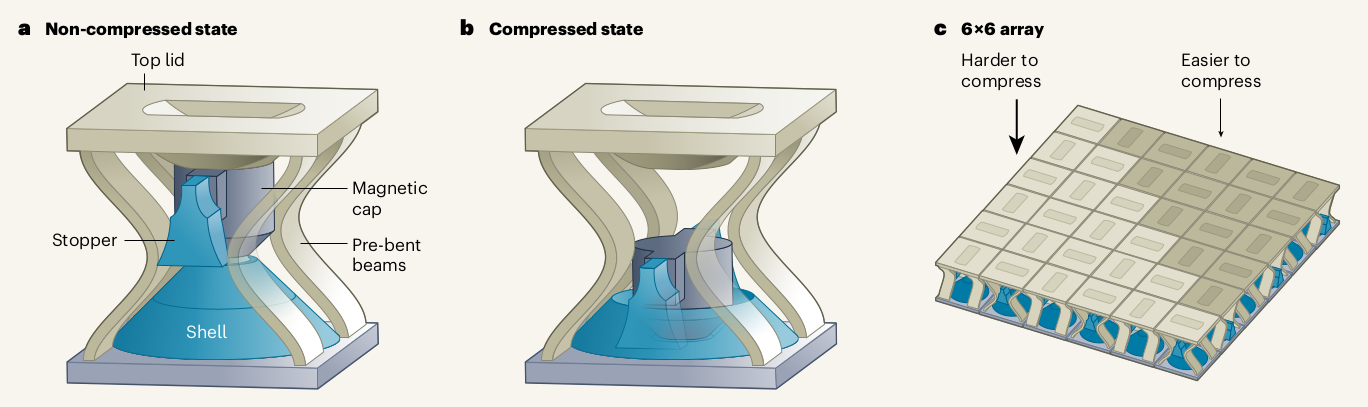
\includegraphics[width=1\textwidth]{shell-work.png}
        %\caption{.}
    \end{figure}
    \small
    A tampa magnética conduz o processo de encaixe, este que por sua vez determina a compressibilidade do ponto. 
%*----------- notes
    \note[item]{Notes can help you to remember important information. Turn on the notes option.}
\end{frame}

\begin{frame}[t]{Unidade básica de armazenamento}
    \transboxout[duration=0.5]
    \framesubtitle{Processo de gravação}
    \begin{columns}
        % \column{.1\textwidth}
        \column{.4\textwidth}
            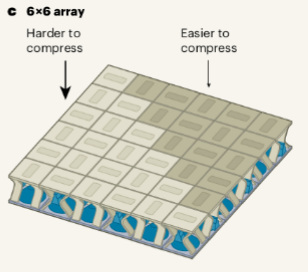
\includegraphics[width=.87\textwidth]{shell-array.png}
        \column{.5\textwidth}
        Utilizando um dispositivo com cabeçote eletromagnético.
            \begin{enumerate}
                \item Percorre a matriz
                \item Encontra o \textit{bit} desejado
                \item Através de indução, define o estado daquele \textit{bit}
            
            \end{enumerate}
        
    \end{columns}
    
    \note[item]{Desse modo, é possível determinar o estado de diferentes partes de um material. Além disso, determina também quanta energia ele pode armazenar.}
\end{frame}
\begin{frame}[t]{Metamateriais}
    \transboxout[duration=0.5]
    \begin{columns}
        \column{.1\textwidth}
        \column{.4\textwidth}
            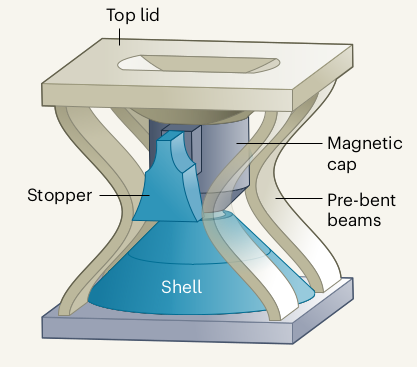
\includegraphics[width=.87\textwidth]{shell.png}
        \column{.6\textwidth}
            \begin{itemize}
                \item Formado por sub-unidades projetadas
                \item Propriedade não encontradas em materiais naturais
            
            \end{itemize}
    \end{columns}
    
    \note[item]{O objeto de estudo é um exemplo de metamaterial.}
\end{frame}
\begin{frame}[t]{Conclusão}
    \transboxout[duration=0.5]
    \framesubtitle{Inovações} 

O dispositivo apresentou a capacidade:
\begin{itemize}
    \item Manipular informações e armazená-las permanentemente
    \item Bits definindo propriedades mecânicas
    \item O estado dos bits poder ser controlados remotamente por campos magnéticos 
\end{itemize}
\only<2->{
    \begin{alertblock}{}
        Nunca antes um dispositivo demonstrou ter estas duas propriedades simultâneamente.
    \end{alertblock}

}
 %*----------- notes
    \note[item]{Notes can help you to remember important information. Turn on the notes option.}
\end{frame}



\begin{frame}[t]{Conclusão}
    \transboxout[duration=0.5]
    \framesubtitle{Limitações} 
    \begin{itemize}
        \item Geometria complexa
        \item Complexidade na fabricação
        \item Densidade de armazenamento
    \end{itemize}
    \begin{figure}
        \begin{figure}[H]
            \centering
            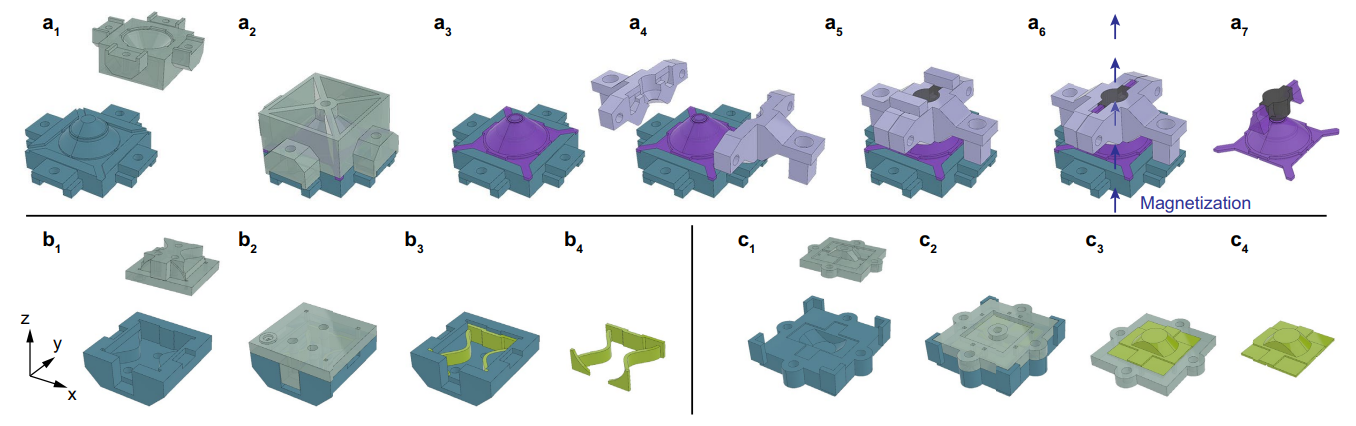
\includegraphics[width = 0.7\textwidth]{source/pictures/fabrication.png}
            \caption{Processo de fabricação\cite{chen2021reprogrammable}.}
            \label{fig:uba-fabrication}
        \end{figure}
        %\caption{.}
    \end{figure}
    \small
\end{frame}


\begin{frame}{Conclusão}
    \framesubtitle{Aplicações}
    
    \centering % Para centralizarmos o vídeo
    \includemedia[
    label=nome_qualquer, % ! Importante para linkar o vídeo ao botão (ver abaixo)
    width=0.6\linewidth, height=0.375\linewidth, % Dimensões
    addresource=./source/movies/compress-material.mp4, % ESTE É O SEU ARQUIVO DE VÍDEO (mesmo dir.)
    transparent, % Opções para que o player tenha transparência
    activate=pageopen, % Se você deseja que o vídeo esteja "carregado" ao abrir a página
    flashvars={
    source=./source/movies/compress-material.mp4
    &loop=true % Se você quer que o vídeo repita automaticamente 
    &scaleMode=letterbox % Manter proporções (dimensionais) do vídeo
    }
    ]{}{VPlayer.swf}
    \vspace{1cm} % Espaçamento entre vídeo e botão
    
    % Agora, você cria o botão para dar play/pause. Neste caso, o botão é apenas a letra "pi".
    
    \mediabutton[
    mediacommand=nome_qualquer:playPause,
    overface=\color{black}{{\strut $\pi$}},
    downface=\color{gray}{{\strut $\pi$}}
    ]{{\strut $\pi$}}
    
    
\end{frame}



\begin{frame}[t]{Conclusão}
    \transboxout[duration=0.5]
    \framesubtitle{Mapa conceitual}    %\transboxin[duration=1,direction=30]

    \begin{figure}
        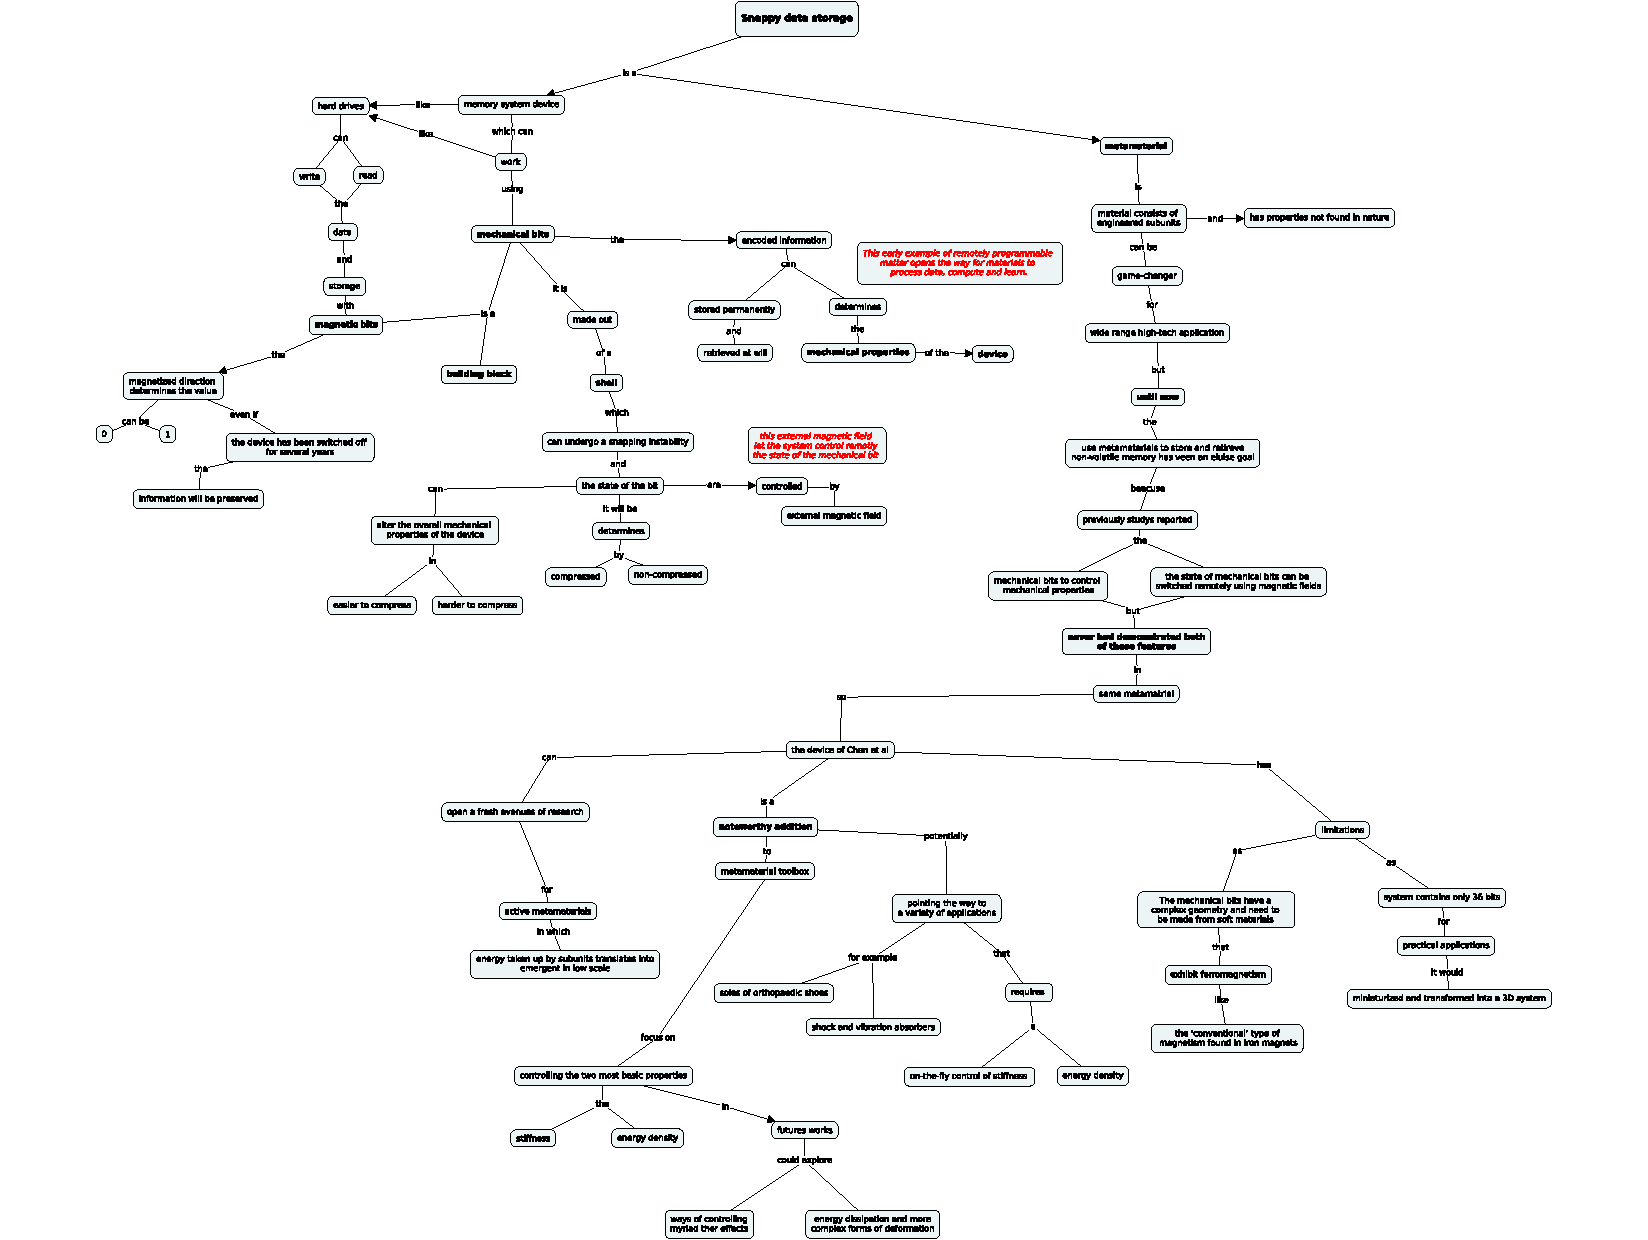
\includegraphics[width=0.55\textwidth]{concept-map.pdf}
        %\caption{.}
    \end{figure}
%*----------- notes
\end{frame}

%----------------------------------------------------SLIDE------------------
 \begin{frame}[t, allowframebreaks]{References}
 %\frametitle{References}
%\begin{frame}{Reference}
    %\transboxin[duration=1,direction=30]

    % \begin{bibunit}[plain]
    % %\cite{kanakia2012}
    % %\cite{agostini2007}
    % %\cite{azuma1997survey}
    % \cite{Buss2005}
  
    % \putbib
    % \end{bibunit}
  
    %\bibliographystyle{IEEEtran}
    %\bibliographystyle{IEEEtranS}
    %\bibliographystyle{IEEEbib}
    \bibliographystyle{abntex2-alf}
    %\bibliographystyle{abntex2-num}
    %\bibliographystyle{abnt-alf}
    \bibliography{bibliography} 
    %\putbib

%*----------- notes
    %\note[item]{Notes can help you to remember important information. Turn on the notes option.}
\end{frame}
%-
%*----------- SLIDE-BACKUP ------------------------------------------------------
% \backupbegin
% %
% \begin{frame}{Backup}
%     Test
% %*----------- notes-------------------------------
% \note{Notes can help you to remember important information. Turn on the notes option.}
% \end{frame}
% %-
% \backupend
% %-
%*----------- QUESTIONS ---------------------------------------------------------
\begin{frame}[c,plain]
    \lastpage{
        \begin{center}   
            {\usebeamerfont{title} Questions?}\\[3ex] 
            %\hspace{1.5cm} 
            vitormendesrb@gmail.com
        \end{center}
    }
    
    %*----------- notes---------------------------------
    \note[item]{Notes can help you to remember important information. Turn on the notes option.}
\end{frame}
%*-------------------------------------------------------------------------------
\end{document}